%% Flowchart of the proposed procedure (companion to Algorithm 1).
\documentclass[border=3pt]{standalone}
\usepackage{amsmath,amssymb}
\usepackage{tikz}
\usetikzlibrary{calc,arrows.meta,positioning,shapes.geometric,shapes.misc,shadows.blur}
%% Simple vector icons drawn with TikZ primitives (original artwork, no external icon set).
%% Each icon fits roughly in [-0.5,0.5]^2; use  \pic[scale=..] at (x,y) {name=colour};
\tikzset{
  ic/.style={line width=0.6pt, line cap=round, line join=round},
  % ---- clipboard / survey
  pics/survey/.style={code={
    \draw[ic,#1,fill=#1!10,rounded corners=1.5pt] (-0.34,-0.46) rectangle (0.34,0.40);
    \draw[ic,#1,fill=#1!60,rounded corners=1pt] (-0.13,0.34) rectangle (0.13,0.48);
    \foreach \y in {0.18,-0.04,-0.26}{
      \draw[ic,#1] (-0.24,\y) -- (-0.18,\y-0.05) -- (-0.08,\y+0.06);
      \draw[ic,#1!70] (0.0,\y) -- (0.24,\y);}
  }},
  % ---- wind turbine
  pics/turbine/.style={code={
    \fill[#1!70] (-0.035,-0.5) -- (0.035,-0.5) -- (0.018,0.12) -- (-0.018,0.12) -- cycle;
    \foreach \a in {90,210,330}{
      \fill[#1,rotate around={\a:(0,0.14)}] (0,0.14) .. controls (0.05,0.24) and (0.04,0.40) .. (0,0.48)
            .. controls (-0.025,0.40) and (-0.03,0.24) .. (0,0.14);}
    \fill[white] (0,0.14) circle (0.035); \draw[ic,#1] (0,0.14) circle (0.035);
    \draw[ic,#1!60] (-0.3,-0.5) -- (0.3,-0.5);
  }},
  % ---- solar panel with sun
  pics/solar/.style={code={
    \fill[#1!15,draw=#1,ic] (-0.42,-0.30) -- (0.22,-0.30) -- (0.38,0.06) -- (-0.26,0.06) -- cycle;
    \foreach \t in {0.25,0.5,0.75}{
      \draw[#1,line width=0.4pt] ($(-0.42,-0.30)!\t!(0.22,-0.30)$) -- ($(-0.26,0.06)!\t!(0.38,0.06)$);}
    \draw[#1,line width=0.4pt] (-0.34,-0.12) -- (0.30,-0.12);
    \draw[ic,#1] (-0.05,-0.30) -- (-0.05,-0.46) (-0.18,-0.46) -- (0.08,-0.46);
    \fill[orange!90!yellow] (0.30,0.34) circle (0.09);
    \foreach \a in {0,45,...,315}{\draw[orange!90!yellow,line width=0.5pt] ($(0.30,0.34)+(\a:0.12)$) -- ($(0.30,0.34)+(\a:0.17)$);}
  }},
  % ---- factory with CO2 cloud
  pics/factory/.style={code={
    \fill[#1!15,draw=#1,ic] (-0.46,-0.46) -- (-0.46,-0.06) -- (-0.26,0.06) -- (-0.26,-0.06) -- (-0.06,0.06) -- (-0.06,-0.06)
          -- (0.14,0.06) -- (0.14,0.26) -- (0.26,0.26) -- (0.26,-0.46) -- cycle;
    \foreach \x in {-0.38,-0.20,-0.02}{\fill[#1!60] (\x,-0.30) rectangle (\x+0.09,-0.20);}
    \fill[gray!45] (0.22,0.34) circle (0.07) (0.32,0.40) circle (0.09) (0.44,0.36) circle (0.07) (0.33,0.30) circle (0.07);
    \node[font=\sffamily\bfseries,scale=0.32,text=black!70] at (0.33,0.36) {CO$_2$};
    \draw[ic,#1!60] (-0.5,-0.46) -- (0.34,-0.46);
  }},
  % ---- calendar
  pics/calendar/.style={code={
    \draw[ic,#1,fill=white,rounded corners=1.5pt] (-0.42,-0.42) rectangle (0.42,0.34);
    \fill[#1,rounded corners=1.5pt] (-0.42,0.16) rectangle (0.42,0.34);
    \foreach \x in {-0.22,0.22}{\draw[ic,#1!60!black,line width=1pt] (\x,0.28) -- (\x,0.44);}
    \foreach \i in {0,...,3}{\foreach \j in {0,1,2}{
      \pgfmathsetmacro{\px}{-0.27+\i*0.18}\pgfmathsetmacro{\py}{0.02-\j*0.15}
      \fill[#1!30] (\px,\py) circle (0.045);}}
    \foreach \i/\j in {0/0,2/0,0/2,2/2}{\pgfmathsetmacro{\px}{-0.27+\i*0.18}\pgfmathsetmacro{\py}{0.02-\j*0.15}
      \fill[#1] (\px,\py) circle (0.05);}
  }},
  % ---- gauge (normalisation)
  pics/gauge/.style={code={
    \fill[#1!12] (-0.44,-0.18) arc (180:0:0.44) -- cycle;
    \draw[ic,#1,line width=1.4pt] (-0.44,-0.18) arc (180:0:0.44);
    \foreach \a in {180,150,...,0}{\draw[#1,line width=0.5pt] ($(0,-0.18)+(\a:0.34)$) -- ($(0,-0.18)+(\a:0.42)$);}
    \draw[ic,black!75,line width=0.9pt] (0,-0.18) -- ++(55:0.34);
    \fill[black!75] (0,-0.18) circle (0.05);
    \node[font=\sffamily,scale=0.35] at (-0.38,-0.30) {0}; \node[font=\sffamily,scale=0.35] at (0.38,-0.30) {1};
  }},
  % ---- balance scale (weights)
  pics/balance/.style={code={
    \draw[ic,#1,line width=1pt] (0,-0.42) -- (0,0.34); \draw[ic,#1,line width=1pt] (-0.18,-0.44) -- (0.18,-0.44);
    \draw[ic,#1,line width=1pt,rotate around={-8:(0,0.28)}] (-0.40,0.28) -- (0.40,0.28);
    \fill[#1] (0,0.34) circle (0.045);
    \begin{scope}[rotate around={-8:(0,0.28)}]
      \draw[ic,#1] (-0.40,0.28) -- (-0.50,0.02) (-0.40,0.28) -- (-0.30,0.02);
      \fill[#1!30,draw=#1,ic] (-0.52,0.02) arc (180:360:0.12 and 0.07) -- cycle;
      \draw[ic,#1] (0.40,0.28) -- (0.30,0.02) (0.40,0.28) -- (0.50,0.02);
      \fill[#1!30,draw=#1,ic] (0.28,0.02) arc (180:360:0.12 and 0.07) -- cycle;
    \end{scope}
  }},
  % ---- podium
  pics/podium/.style={code={
    \fill[#1] (-0.14,-0.44) rectangle (0.14,0.10); \fill[#1!65] (-0.44,-0.44) rectangle (-0.14,-0.08);
    \fill[#1!40] (0.14,-0.44) rectangle (0.44,-0.18);
    \node[font=\sffamily\bfseries,white,scale=0.55] at (0,-0.10) {1};
    \node[font=\sffamily\bfseries,white,scale=0.5] at (-0.29,-0.25) {2};
    \node[font=\sffamily\bfseries,white,scale=0.5] at (0.29,-0.31) {3};
    \fill[orange!90!yellow] (0,0.30) -- (0.045,0.22) -- (0.13,0.21) -- (0.065,0.15) -- (0.08,0.06) -- (0,0.105)
          -- (-0.08,0.06) -- (-0.065,0.15) -- (-0.13,0.21) -- (-0.045,0.22) -- cycle;
  }},
  % ---- globe
  pics/globe/.style={code={
    \fill[#1!12] (0,0) circle (0.44); \draw[ic,#1] (0,0) circle (0.44);
    \draw[ic,#1] (0,-0.44) arc (-90:90:0.18 and 0.44) (0,-0.44) arc (270:90:0.18 and 0.44) (0,-0.44) -- (0,0.44);
    \draw[ic,#1] (-0.44,0) -- (0.44,0); \draw[ic,#1] (-0.39,0.2) -- (0.39,0.2) (-0.39,-0.2) -- (0.39,-0.2);
  }},
  % ---- shield with check
  pics/shield/.style={code={
    \fill[#1!15,draw=#1,ic] (0,0.46) -- (0.38,0.32) -- (0.36,-0.05) .. controls (0.30,-0.30) and (0.12,-0.40) .. (0,-0.47)
          .. controls (-0.12,-0.40) and (-0.30,-0.30) .. (-0.36,-0.05) -- (-0.38,0.32) -- cycle;
    \draw[ic,#1,line width=1.3pt] (-0.16,0.0) -- (-0.04,-0.13) -- (0.18,0.14);
  }},
  % ---- magnifier
  pics/magnifier/.style={code={
    \fill[#1!12] (-0.08,0.08) circle (0.28); \draw[ic,#1,line width=1.3pt] (-0.08,0.08) circle (0.28);
    \draw[#1,line width=3pt,line cap=round] (0.13,-0.13) -- (0.40,-0.40);
    \draw[ic,#1!70] (-0.22,0.02) -- (-0.14,0.14) -- (-0.04,0.06) -- (0.06,0.20);
  }},
  % ---- dice
  pics/dice/.style={code={
    \fill[#1!12,draw=#1,ic,rounded corners=3pt] (-0.40,-0.40) rectangle (0.40,0.40);
    \foreach \p in {(-0.2,0.2),(0.2,0.2),(0,0),(-0.2,-0.2),(0.2,-0.2)}{\fill[#1] \p circle (0.065);}
  }},
  % ---- target
  pics/target/.style={code={
    \fill[#1!12,draw=#1,ic] (0,0) circle (0.44); \fill[#1!35,draw=#1,ic] (0,0) circle (0.31);
    \fill[#1!12,draw=#1,ic] (0,0) circle (0.18);
    \fill[#1] (0,0) circle (0.07);
    \draw[ic,black!75,line width=0.9pt,-{Stealth[length=3pt]}] (0.46,0.46) -- (0.06,0.06);
  }},
  % ---- light bulb
  pics/bulb/.style={code={
    \fill[#1!15,draw=#1,ic] (-0.10,-0.18) .. controls (-0.12,-0.02) and (-0.28,0.04) .. (-0.28,0.18) arc (180:0:0.28)
          .. controls (0.28,0.04) and (0.12,-0.02) .. (0.10,-0.18) -- cycle;
    \fill[#1!70] (-0.11,-0.22) rectangle (0.11,-0.30); \fill[#1!70] (-0.09,-0.33) rectangle (0.09,-0.40);
    \draw[ic,#1] (-0.06,-0.18) -- (-0.04,0.10) -- (0,0.04) -- (0.04,0.10) -- (0.06,-0.18);
    \foreach \a in {20,55,90,125,160}{\draw[ic,orange!90!yellow] ($(0,0.18)+(\a:0.36)$) -- ($(0,0.18)+(\a:0.46)$);}
  }},
  % ---- document (literature)
  pics/document/.style={code={
    \fill[white,draw=#1,ic] (-0.32,-0.44) -- (-0.32,0.44) -- (0.16,0.44) -- (0.32,0.28) -- (0.32,-0.44) -- cycle;
    \fill[#1!30,draw=#1,ic] (0.16,0.44) -- (0.16,0.28) -- (0.32,0.28) -- cycle;
    \foreach \y in {0.22,0.08,-0.06,-0.20,-0.34}{\draw[ic,#1!70] (-0.22,\y) -- (0.22,\y);}
  }},
  % ---- speech bubble with question mark
  pics/question/.style={code={
    \fill[#1!15,draw=#1,ic,rounded corners=4pt] (-0.44,-0.22) rectangle (0.44,0.42);
    \fill[#1!15,draw=#1,ic] (-0.20,-0.215) -- (-0.30,-0.44) -- (-0.02,-0.215);
    \node[font=\sffamily\bfseries,text=#1,scale=0.9] at (0,0.10) {?};
  }},
  % ---- gear
  pics/gear/.style={code={
    \foreach \a in {0,45,...,315}{\fill[#1,rotate=\a] (-0.07,0.30) rectangle (0.07,0.44);}
    \fill[#1] (0,0) circle (0.33); \fill[white] (0,0) circle (0.13);
  }},
}

\definecolor{cData}{HTML}{16877F}
\definecolor{cProc}{HTML}{3B5BA5}
\definecolor{cWeight}{HTML}{D08414}
\definecolor{cRank}{HTML}{2E8B57}
\definecolor{cDec}{HTML}{C0503F}
\definecolor{cInk}{HTML}{2D3748}
\newcommand{\figtiny}{\fontsize{6}{7}\selectfont}
\begin{document}
\sffamily\hyphenpenalty=10000
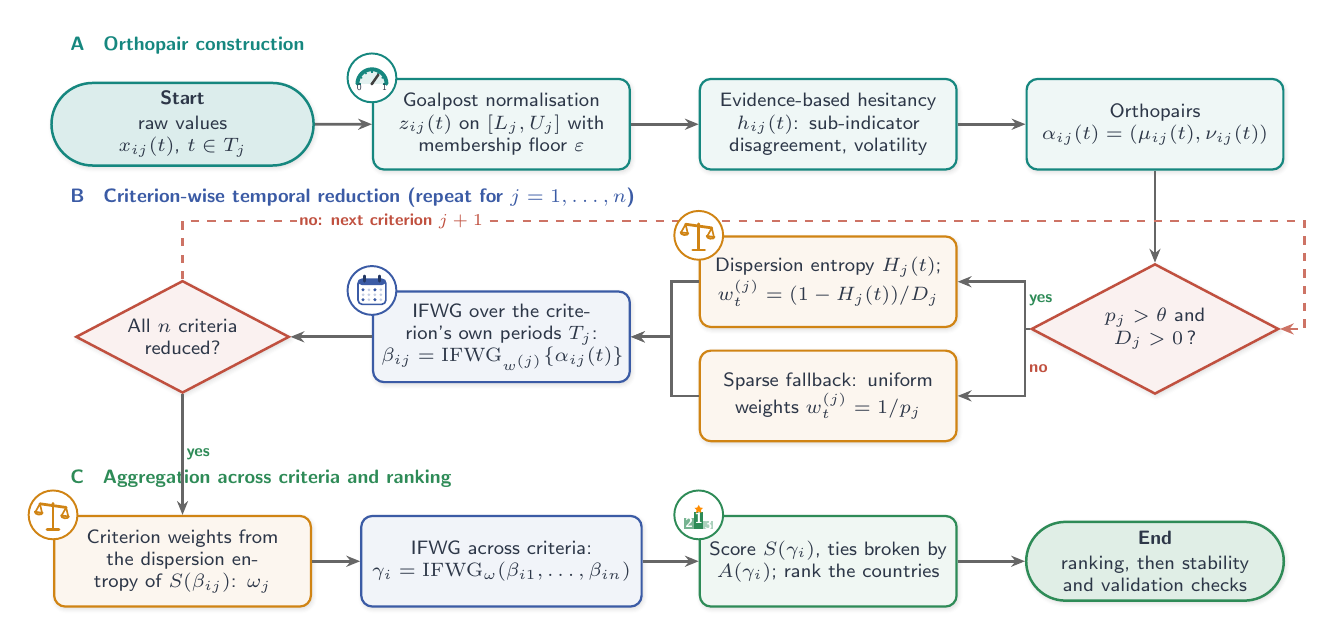
\begin{tikzpicture}[font=\sffamily\scriptsize, text=cInk, >={Stealth[length=5pt,width=4pt]},
  shadow/.style={blur shadow={shadow blur steps=5, shadow xshift=0.5pt, shadow yshift=-0.8pt, shadow opacity=16}},
  box/.style={rectangle, rounded corners=4pt, draw=#1, line width=0.8pt, fill=#1!7, align=center,
              text width=3.05cm, minimum height=1.15cm, inner sep=3pt, shadow},
  term/.style={rounded rectangle, draw=#1, line width=0.9pt, fill=#1!15, align=center, text width=2.7cm,
               minimum height=1.0cm, inner sep=3pt, shadow, font=\sffamily\bfseries\scriptsize},
  dec/.style={diamond, aspect=1.9, draw=cDec, line width=0.9pt, fill=cDec!8, align=center, inner sep=0.5pt,
              text width=2.05cm, shadow, font=\sffamily\scriptsize},
  line/.style={->, line width=1pt, color=black!60},
  lab/.style={font=\sffamily\bfseries\figtiny, text=#1, fill=white, inner sep=1pt},
  stage/.style={font=\sffamily\bfseries\scriptsize, text=#1, anchor=west},
]
% ---------------------------------------------------------------- stage labels
\node[stage=cData] at (0,6.55) {A\;\; Orthopair construction};
\node[stage=cProc] at (0,4.62) {B\;\; Criterion-wise temporal reduction (repeat for $j=1,\dots,n$)};
\node[stage=cRank] at (0,1.05) {C\;\; Aggregation across criteria and ranking};
% ---------------------------------------------------------------- row A
\node[term=cData] (start) at (1.55,5.55) {Start\\[1pt]\mdseries raw values \mbox{$x_{ij}(t)$, $t\in T_j$}};
\node[box=cData] (norm) at (5.60,5.55) {Goalpost normalisation\\ $z_{ij}(t)$ on $[L_j,U_j]$ with membership floor $\varepsilon$};
\node[box=cData] (hes) at (9.75,5.55) {Evidence-based hesitancy $h_{ij}(t)$: sub-indicator disagreement, volatility};
\node[box=cData] (orth) at (13.90,5.55) {Orthopairs\\ \mbox{$\alpha_{ij}(t)=(\mu_{ij}(t),\nu_{ij}(t))$}};
\draw[line] (start) -- (norm); \draw[line] (norm) -- (hes); \draw[line] (hes) -- (orth);
% ---------------------------------------------------------------- row B
\node[dec] (d1) at (13.90,2.95) {\mbox{$p_j>\theta$ and}\\ \mbox{$D_j>0$\,?}};
\node[box=cWeight] (ent) at (9.75,3.55) {Dispersion entropy $H_j(t)$;\\ \mbox{$w^{(j)}_t=(1-H_j(t))/D_j$}};
\node[box=cWeight] (uni) at (9.75,2.10) {Sparse fallback: uniform\\ weights \mbox{$w^{(j)}_t=1/p_j$}};
\node[box=cProc] (red) at (5.60,2.85) {IFWG over the criterion's own periods $T_j$:\\ \mbox{$\beta_{ij}=\mathrm{IFWG}_{w^{(j)}}\{\alpha_{ij}(t)\}$}};
\node[dec, text width=1.75cm] (d2) at (1.55,2.85) {All $n$ criteria reduced?};
\draw[line] (orth) -- (d1);
\coordinate (split) at (12.25,2.95);
\draw[line, -] (d1.west) -- (split);
\draw[line] (split) |- (ent.east) node[lab=cRank, pos=0.30, right] {yes};
\draw[line] (split) |- (uni.east) node[lab=cDec, pos=0.30, right] {no};
\draw[line] (ent.west) -- ++(-0.35,0) |- (red.east);
\draw[line] (uni.west) -- ++(-0.35,0) |- (red.east);
\draw[line] (red) -- (d2);
\draw[line, dashed, color=cDec!80] (d2.north) -- (1.55,4.32) -- (15.80,4.32) |- (d1.east);
\node[lab=cDec] at (4.2,4.32) {no: next criterion $j+1$};
% ---------------------------------------------------------------- row C
\node[box=cWeight] (cw) at (1.55,0.0) {Criterion weights from the dispersion entropy of $S(\beta_{ij})$: $\omega_j$};
\node[box=cProc, text width=3.35cm] (agg) at (5.60,0.0) {IFWG across criteria:\\ \mbox{$\gamma_i=\mathrm{IFWG}_\omega(\beta_{i1},\dots,\beta_{in})$}};
\node[box=cRank] (rank) at (9.75,0.0) {Score $S(\gamma_i)$, ties broken by $A(\gamma_i)$; rank the countries};
\node[term=cRank] (end) at (13.90,0.0) {End\\[1pt]\mdseries ranking, then stability and validation checks};
\draw[line] (d2.south) -- (cw.north) node[lab=cRank, midway, right] {yes};
\draw[line] (cw) -- (agg); \draw[line] (agg) -- (rank); \draw[line] (rank) -- (end);
% ---------------------------------------------------------------- icons
\foreach \n/\ic/\c in {norm/gauge/cData, ent/balance/cWeight, red/calendar/cProc, cw/balance/cWeight, rank/podium/cRank}{
  \node[circle, fill=white, draw=\c, line width=0.7pt, minimum size=0.62cm, inner sep=0pt] at (\n.north west) {};
  \pic[scale=0.42] at (\n.north west) {\ic=\c};}
\end{tikzpicture}
\end{document}
